\section{Continuation states and present-state fibers}
\label{sec:state-space}

A point value \(X(t)\in\mathbb{R}^d\) is not, by itself, a Markov state for a Caputo equation. We therefore formulate basin membership on the continuation-state space associated with autonomous Caputo semidynamical systems. Consider
\begin{equation}
  \CapD X(t)=g(X(t)),
  \qquad 0<\alpha<1,
  \label{eq:caputo-general}
\end{equation}
on a physical state domain \(X_{\mathrm{phys}}\subset\mathbb{R}^d\). Following the continuation-state construction of Doan and Kloeden
\cite{DoanKloeden2021Semidynamical,DoanKloeden2024Attractors}, let
\[
  \Cspace=C(\mathbb{R}_+,\mathbb{R}^d).
\]
For
\[
  \|f-h\|_n
  :=
  \sup_{0\le\tau\le n}\|f(\tau)-h(\tau)\|,
\]
we use the compatible compact-open metric
\begin{equation}
  \rho_{\Cspace}(f,h)
  =
  \sum_{n=1}^{\infty}
  2^{-n}
  \frac{\|f-h\|_n}{1+\|f-h\|_n}.
  \label{eq:compact-open-metric}
\end{equation}
Let \(T_t\) denote the induced semidynamical system.  For an invariant compact set \(A\subset\Cspace\), its basin is
\begin{equation}
  \Basin(A)
  :=
  \left\{
  f\in\Cspace:
  \operatorname{dist}_{\rho_{\Cspace}}(T_tf,A)\to0
  \text{ as }t\to\infty
  \right\}.
  \label{eq:basin-definition}
\end{equation}

For a point initial value \(z\in X_{\mathrm{phys}}\), define the canonical cold-start state
\[
  \iota(z)(\tau)\equiv z,
\]
and define the present evaluation
\[
  e_0(f)=f(0),
  \qquad f\in\Cspace.
\]
The physically reachable subset of \(\Cspace\) is
\begin{equation}
  \Reach
  =
  \{T_t\iota(p):p\in X_{\mathrm{phys}},\ t\ge0\}.
  \label{eq:reachable-set}
\end{equation}

\begin{definition}[Reachable present-state fiber]
\label{def:reachable-fiber}
For \(z\in X_{\mathrm{phys}}\), the physically reachable present-state fiber above \(z\) is
\begin{equation}
  \Fiber{z}
  =
  e_0^{-1}(z)\cap\Reach.
  \label{eq:fiber}
\end{equation}
If \(\Fiber{z}\) intersects two distinct asymptotic basins in \(\Cspace\), we call \(\Fiber{z}\) \emph{multibasin}.
\end{definition}

The definition separates two distinct notions: a present physical value \(z\), and the continuation state that carries the inherited Caputo memory. The central theorem of this paper concerns basin membership inside a single fiber \(\Fiber{z}\), not trajectory intersection by itself.

\begin{figure}[t]
  \centering
  \resizebox{\textwidth}{!}{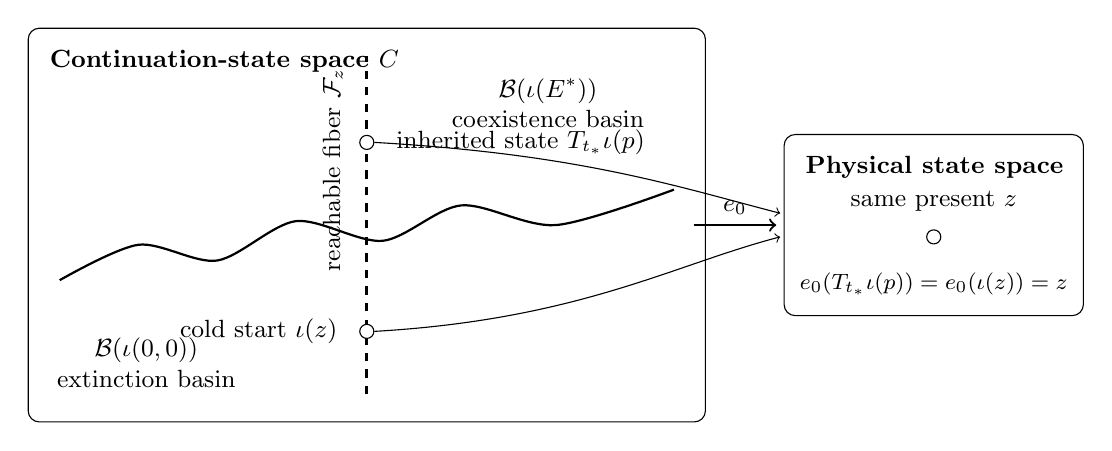
\begin{tikzpicture}[
  x=1cm,y=1cm,
  every node/.style={font=\small},
  state/.style={circle,draw,fill=white,inner sep=1.8pt},
  lab/.style={align=center}
]
  % Continuation-state space
  \draw[rounded corners] (0,0) rectangle (8.6,5.0);
  \node[anchor=north west,font=\small\bfseries] at (0.15,4.85)
    {Continuation-state space \(\mathfrak C\)};

  % Basin separator and labels
  \draw[thick] plot[smooth] coordinates {
    (0.4,1.8) (1.4,2.25) (2.4,2.05) (3.4,2.55)
    (4.5,2.30) (5.5,2.75) (6.7,2.50) (8.2,2.95)
  };
  \node[lab] at (1.5,0.75) {\(\mathcal B(\iota(0,0))\)\\extinction basin};
  \node[lab] at (6.6,4.05) {\(\mathcal B(\iota(E^*))\)\\coexistence basin};

  % Present-state fiber
  \draw[dashed,very thick] (4.3,0.35) -- (4.3,4.65);
  \node[anchor=south,rotate=90] at (4.12,3.2)
    {reachable fiber \(\mathcal F_z\)};

  % Two states in same fiber
  \node[state] (cold) at (4.3,1.15) {};
  \node[anchor=east] at (4.05,1.15)
    {cold start \(\iota(z)\)};

  \node[state] (inh) at (4.3,3.55) {};
  \node[anchor=west] at (4.55,3.55)
    {inherited state \(T_{t_*}\iota(p)\)};

  % Physical state space at right
  \draw[rounded corners] (9.6,1.35) rectangle (13.4,3.65);
  \node[anchor=north west,font=\small\bfseries] at (9.75,3.5)
    {Physical state space};
  \node[state] (z) at (11.5,2.35) {};
  \node[anchor=south] at (11.5,2.55)
    {same present \(z\)};

  % Evaluation projection
  \draw[->,thick] (8.45,2.5) -- node[above] {\(e_0\)} (9.5,2.5);
  \draw[->,thin] (inh.east) .. controls (7.0,3.4) and (8.2,3.0) .. (9.55,2.65);
  \draw[->,thin] (cold.east) .. controls (7.0,1.3) and (8.2,2.0) .. (9.55,2.35);

  % Caption-like logical statement within figure
  \node[align=center,font=\footnotesize] at (11.5,1.75)
    {\(e_0(T_{t_*}\iota(p))=e_0(\iota(z))=z\)};
\end{tikzpicture}
}
  \caption{Geometry of a multibasin reachable present-state fiber.  The inherited continuation state and the canonical cold start have the identical present evaluation \(z\), but lie in different basins in the continuation-state space.  The diagram is schematic; the existence of this configuration is proved in \cref{thm:principal}.}
  \label{fig:fiber-geometry}
\end{figure}

\begin{proposition}[Physical convergence lifts to continuation-state convergence]
\label{prop:physical-to-continuation}
Let \(X(\cdot;p)\) be the standard point-IVP solution of \eqref{eq:caputo-general}. If
\[
  X(t;p)\to X^*,
  \qquad
  g(X^*)=0,
\]
then
\[
  T_t\iota(p)\to\iota(X^*)
\]
in the compact-open topology of \(\Cspace\).
\end{proposition}

\begin{proof}
Fix \(N>0\) and \(0\le\eta\le N\). By the continuation-state formula,
\[
  (T_t\iota(p))(\eta)
  =
  p+
  \frac{1}{\Gamma(\alpha)}
  \int_0^t
  (t+\eta-s)^{\alpha-1}g(X(s;p))\,ds.
\]
On the other hand,
\[
  X(t+\eta;p)
  =
  p+
  \frac{1}{\Gamma(\alpha)}
  \int_0^{t+\eta}
  (t+\eta-s)^{\alpha-1}g(X(s;p))\,ds.
\]
Subtracting gives
\begin{align*}
  (T_t\iota(p))(\eta)-X^*
  &=
  X(t+\eta;p)-X^* \\
  &\quad-
  \frac{1}{\Gamma(\alpha)}
  \int_t^{t+\eta}
  (t+\eta-s)^{\alpha-1}g(X(s;p))\,ds.
\end{align*}
The first term tends uniformly to zero for \(0\le\eta\le N\). The second satisfies
\[
  \sup_{0\le\eta\le N}
  \left\|
  \frac{1}{\Gamma(\alpha)}
  \int_t^{t+\eta}
  (t+\eta-s)^{\alpha-1}g(X(s;p))\,ds
  \right\|
  \le
  \frac{N^\alpha}{\Gamma(\alpha+1)}
  \sup_{s\ge t}\|g(X(s;p))\|,
\]
which also tends to zero because \(g(X(t;p))\to g(X^*)=0\). Hence
\[
  \sup_{0\le\eta\le N}
  \|(T_t\iota(p))(\eta)-X^*\|\to0
\]
for every \(N\), which is compact-open convergence.
\end{proof}

\begin{proposition}[Basin-entry criterion]
\label{prop:basin-entry}
Let \(A_-\neq A_+\) be invariant asymptotic states or attractors in \(\Cspace\). Suppose
\[
  \iota(U_-)\subset\Basin(A_-),
  \qquad
  \iota(p)\in\Basin(A_+),
\]
for a physical set \(U_-\subset X_{\mathrm{phys}}\). If
\[
  z=X(t_*;p)\in U_-,
\]
then
\[
  T_{t_*}\iota(p),\ \iota(z)\in\Fiber{z},
\]
with
\[
  T_{t_*}\iota(p)\in\Basin(A_+),
  \qquad
  \iota(z)\in\Basin(A_-).
\]
Consequently \(\Fiber{z}\) is multibasin.
\end{proposition}

\begin{proof}
The two states have the same present value:
\[
  e_0(T_{t_*}\iota(p))
  =
  X(t_*;p)
  =
  z
  =
  e_0(\iota(z)).
\]
Both belong to \(\Reach\), so both lie in \(\Fiber{z}\). Basin positive invariance gives
\[
  T_{t_*}\iota(p)\in\Basin(A_+),
\]
while the definition of \(U_-\) gives
\[
  \iota(z)\in\Basin(A_-).
\]
Since \(A_-\neq A_+\), the fiber intersects two distinct basins.
\end{proof}

\begin{corollary}[Nondegenerate time-interval criterion]
\label{cor:time-interval}
Under the hypotheses of \cref{prop:basin-entry}, if
\[
  X(t;p)\in U_-
  \qquad
  \text{for every }t\in I
\]
on a nondegenerate interval \(I\), then
\[
  \Fiber{X(t;p)}
\]
is multibasin for every \(t\in I\).
\end{corollary}

\begin{remark}[Why compact-open topology is essential]
\label{rem:tail-anchoring}
For any fixed \(T>0\), if \(X(\cdot;p)\) is bounded on \([0,T]\), then
\[
  (T_T\iota(p))(\tau)
  =
  p+
  \frac{1}{\Gamma(\alpha)}
  \int_0^T
  (T+\tau-s)^{\alpha-1}g(X(s;p))\,ds
  \to p
\]
as \(\tau\to\infty\). Thus a finite-time continuation state need not be globally close to a terminal equilibrium in the unweighted sup norm, even when the underlying physical trajectory converges. The compact-open topology is therefore not a technical convenience but a structural feature of the continuation-state representation.
\end{remark}
